\documentclass[review]{elsarticle}

\usepackage{lineno,hyperref}
\modulolinenumbers[5]

\journal{Nucl. Instr. Meth. Nucl. in Phys. Res. A}

\bibliographystyle{elsarticle-num}

\begin{document}

\begin{frontmatter}

\title{PLUME in BEAST}

\author[iphc]{D.~Cuesta}
\author[iphc]{J.~Baudot}
\author[iphc]{G.Claus}
\author[iphc]{M.~Goffe}
\author[iphc]{K.~Jaaskelainen}
\author[jsi]{L.~Santelj}
\author[iphc]{M.~Specht}
\author[iphc]{M.~Szelezniak}
\author[iphc]{I.~Ripp-Baudot\corref{corr}}

\address[iphc]{Universit\'e de Strasbourg, CNRS, IPHC UMR 7178, F-67000 Strasbourg, France}
\address[jsi]{J. Stefan Institute, 1000 Ljubljana, Slovenia}

\cortext[corr]{Corresponding author}
\ead{isabelle.ripp-baudot@iphc.cnrs.fr}


\begin{abstract}
This template helps you to create a properly formatted \LaTeX\ manuscript.
\end{abstract}

\begin{keyword}
pixel sensor, CMOS sensor, tracker
\end{keyword}

\end{frontmatter}

\linenumbers

\section{Introduction}
\label{sec:introduction}
{\it intro ~1p  Isabelle\\
     - context and PLUME goals
}

\section{System description}
\label{sec:system}
{\it system description ~2p + 2 figures  Jerome\\
     - sensors, DAQ, services\\
     - data registration (EPICS)\\
     - location wrt BEAST
}

\begin{figure}[!h]
\centering
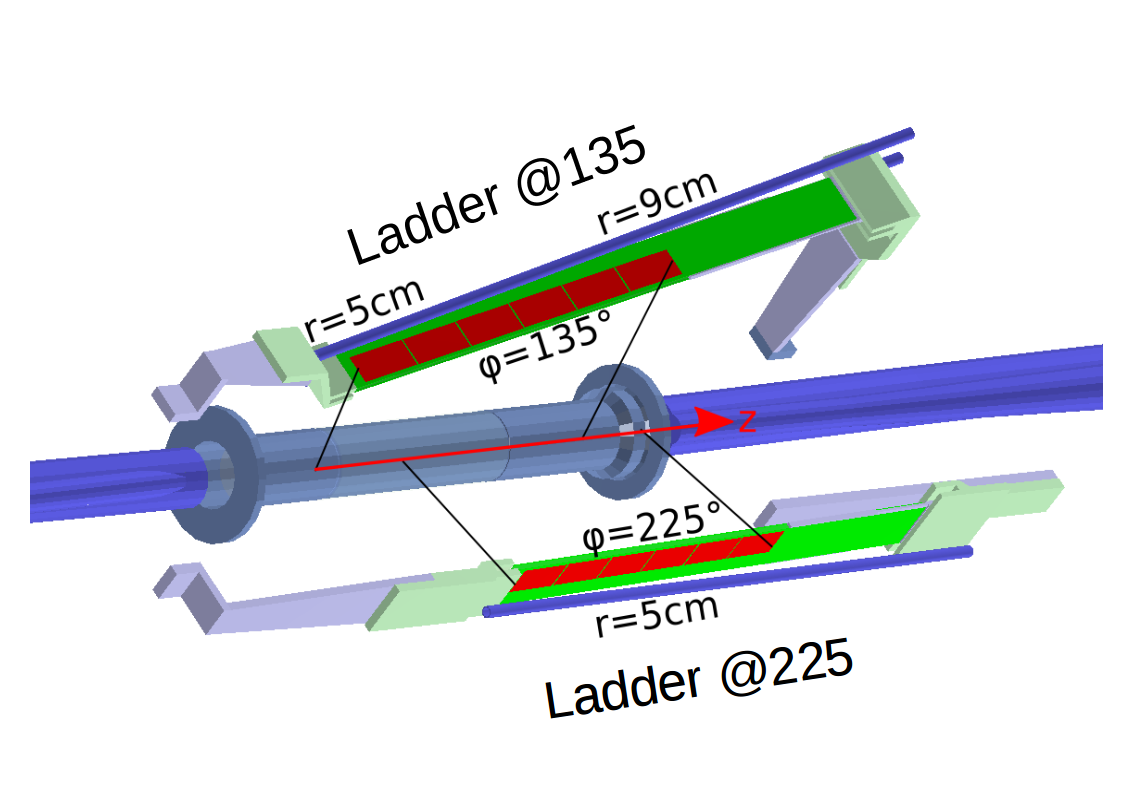
\includegraphics[width=\linewidth]{plumeGeometry_simplified.png}
%\scalebox{0.4}{\input{IMICactivity.tex}}
\caption{Test figure with a PNG format.}
\label{fig:geometry}
\end{figure}

\begin{figure}[!h]
\centering
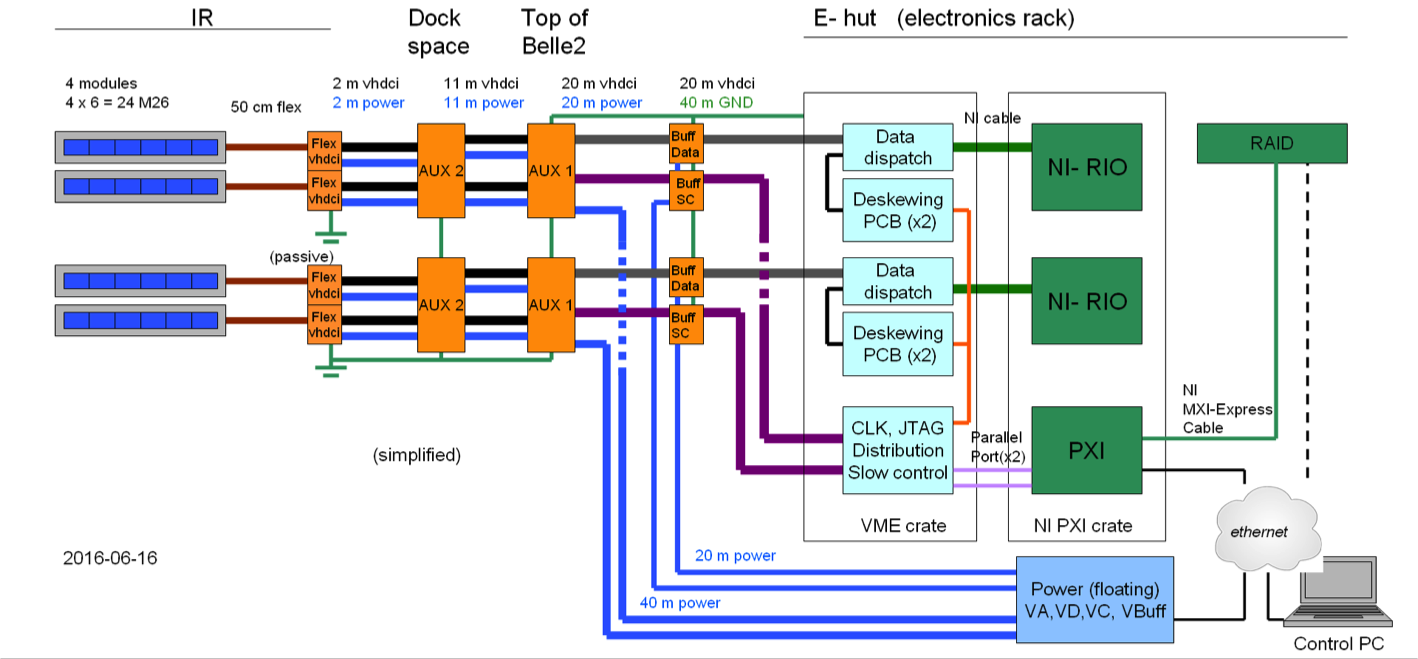
\includegraphics[width=\linewidth]{systemSchematic.png}
%\scalebox{0.4}{\input{IMICactivity.tex}}
\caption{Test figure with a PNG format.}
\label{fig:system}
\end{figure}


\section{Data taking and analysis}
\label{sec:data}
{\it data taking ~2p + 2 figures\\
     - fake rate  Daniel\\
     - cluster  Daniel\\
     - hit rate  Daniel\\
     - history of operation  Isabelle\\
     - main runs for sub-section 4/  Isabelle \\
     - stability / TID Isaabelle
}

\section{Analysis of double-sided feature}
\label{sec:doublesided}
{\it double-sided exploitation ~4p + 4 figures\\
     - use of redundancy in hit rate measurement\\
     - hit-rate difference among two sides\\
     - momentum measurement  Daniel\\
     - lumi background  Daniel\\
}

\section{conclusion}
\label{sec:conclusion}
{\it Conclusion and ref ~ 1p  Isabelle\\    
   o easiness to integrate\\
   o stable operation of PLUME / occupancy / TID\\
   o space investigation of hit-rate\\
   o hit-rate difference between sides and momentum \\
   o lumi background estimate thanks to double-sided
}

\section*{Acknowledgement}
SuperKEKB, BEAST, Belle II, IDEX

\section*{References}
\bibliography{mybibfile}

\end{document}